\FloatBarrier

\begin{figure}[h!]
	\centering
	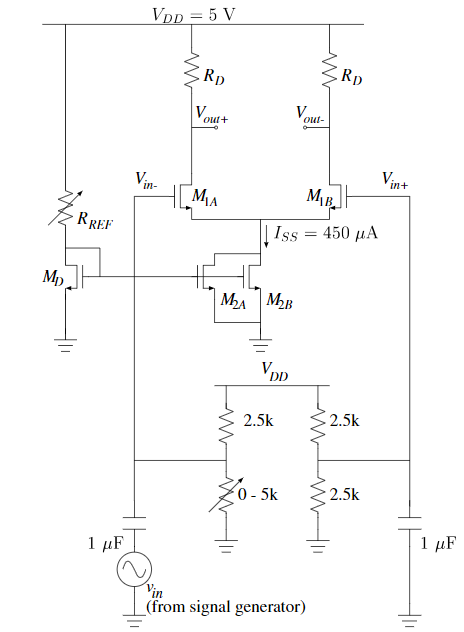
\includegraphics[scale=0.75]{./images/circuit.PNG}
	\caption{Differential Amplifier}
	\label{fig:circuit}
\end{figure}

\FloatBarrier

First, the left hand portion of the current source is constructed.
The resistor $R_{REF}$ is tuned to get the proper $225$\si{\micro\ampere} current.
A $10$\si{\kilo\ohm} resistor is used, which yields a $213$\si{\micro\ampere} current.
The two transistors for the current sources are then attached.
Since each current source is expected to produce $225$\si{\micro\ampere}, the total current $I_{SS}$ is expected to be $450$\si{\micro\ampere}.
Their total current $I_{SS}$ is measured to be about $480$\si{\micro\ampere}, which is quite close.
They are tested by setting the drain voltage sufficiently high so that both of the transistors on the right-hand of the current source enter saturation. \\

The first voltage divider is then constructed and tested with two $5$\si{\kilo\ohm} resistors in series.
Common source amplifiers are constructed with $M_{1A}$ and $M_{1B}$.
$5$\si{\kilo\ohm} and $10$\si{\kilo\ohm} resistors in parallel ($3.3$\si{\kilo\ohm} equivalent resistance) for $R_D$ turn out to be sufficient to ensure that both transistors at the voltage input are biased in the middle of the saturation region, which corresponds to an output voltage of about $3.0$\si{\volt}. \\

The current sources and the two halves of the differential pair are then connected to form the final amplifier.
The bias current on either half of the differential pair is expected to be about $225$\si{\micro\ampere}.
On one side, $240$\si{\micro\ampere} is measured.
On the other side, $246$\si{\micro\ampere} is measured.
These values are astonishingly close to the design specification. \\
